\documentclass[12pt]{article}
\usepackage{xcolor}
\usepackage{graphicx}
%\usepackage{appendix}
%\usepackage{verbatim}
\usepackage[margin=1.0in]{geometry}
\DeclareGraphicsExtensions{.jpg,.jpeg,.png}
\renewcommand{\baselinestretch}{1.0}
\begin{document}
\newcommand{\dt}{\Delta t}
\newcommand{\Fvec}{\overline{F}}
\newcommand{\rvec}{\overline{r}}
\newcommand{\xvec}{\overline{x}}
\newcommand{\Xvec}{\overline{X}}
\newcommand{\yvec}{\overline{y}}
\newcommand{\Yvec}{\overline{Y}}
\newcommand{\Gvec}{\overline{G}}
\newcommand{\svec}{\overline{s}}
\newcommand{\Dmat}{\overline{\overline{D}}}
\newcommand{\Rmat}{\overline{\overline{R}}}
\newcommand{\Imat}{\overline{\overline{I}}}
\newcommand{\Hmat}{\overline{\overline{H}}}
\newcommand{\Lag}{\mathcal{L}}
\title{Simple Model of Cell Growth on a Stationary Nutrient Medium}
\author{Written by a cast of thousands}
\maketitle

% Change table counter
\renewcommand{\thetable}{\Roman{table}}

\section{Model}
This document describes the initial model implemented with the BoltzmannMFX
framework. This model is an extremely simplified model of microbial growth
designed to illustrated how the different components of the BoltzmannMFX
framework fit together and interact with each other. The cells consist of simple
circular disks that form a single layer on top of a stationary growth medium
(e.g. agar) and are fed by a single component ``nutrient''. The cells absorb the
nutrient and grow. When they reach a certain size, they split into two new
cells.

\begin{figure}
\centering
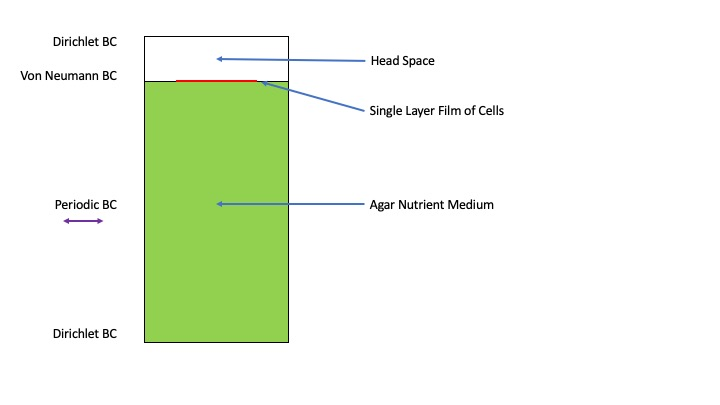
\includegraphics[width=4.0in,keepaspectratio=true]{FullSys}
\caption{\label{fullsys} Schematic diagram of the model growth region.}
\end{figure}
The geometry of the system is illustrated in figure (\ref{fullsys}) and shows a
rectangular volume that is square in cross section and elongated along one axis.
the system is periodic along the short axes. The long axis is divided into two
regions, one consisting of the stationary growth region and the other consisting
of a non-participating ``head-space''. The nutrient concentration is maintained
at a fixed value at the bottom of the system, corresponding to a Dirichlet
boundary condition. The top of the growth medium is impermeable to the nutrient,
so it should be characterized by a Von Neumann boundary condition representing
a zero normal gradient for the nutrient concentration. The head space does not
contain any chemical species and for this problem does not participate in any
significant way. The cells grow on top of the nutrient support layer in a
two-dimensional pattern.

\begin{figure}
\centering
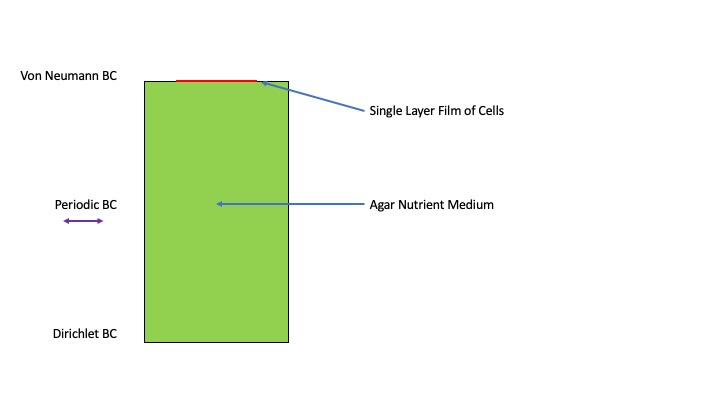
\includegraphics[width=4.0in,keepaspectratio=true]{ReducedSys}
\caption{\label{reducedsys} Schematic diagram of the model growth region with
head space removed.}
\end{figure}
Because the head space does not participate in this
model, it is possible to eliminate it entirely and use the geometry shown in
figure (\ref{reducedsys}). This eliminates an internal boundary and should make
development easier, but may gloss over an issue that will need to be dealt with
later as the model becomes more realistic.

\begin{figure}
\centering
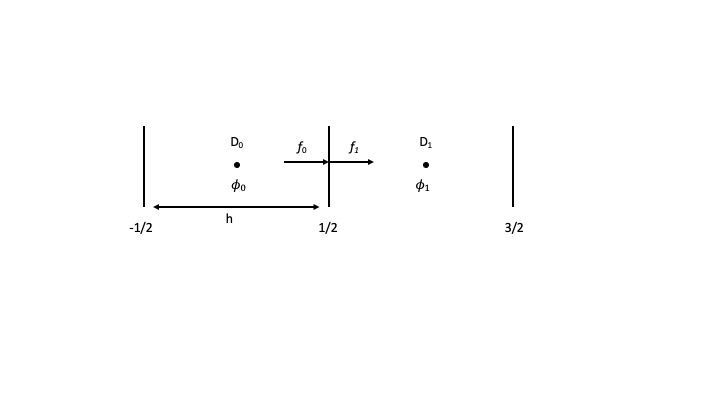
\includegraphics[width=4.0in,keepaspectratio=true]{DiffBC}
\caption{\label{diffbc} Illustration of the geometry for solving the boundary
conditions between two media with different diffusion coefficients.}
\end{figure}
In the case that there is an internal boundary, the finite volume approach can
be used to incorporate the effects of the jump in diffusion coefficient. For
simplicity, consider a 1-dimensional system with evenly spaced grid cells of
size $h$. The centers of the grid cells are indexed by the integers $i$ and the
faces between the cells are indexed by $i+1/2$. Consider two grid cells at $i=0$
and $i=1$ and assume that the boundary between them at $i=1/2$ is where the
diffusion coefficient changes abruptly from the value $D_0$ to $D_1$. The
cell-centered concentration values are $\phi_0$ and $\phi_1$. The system is
illustrated schematically in figure (\ref{diffbc})

To derive the boundary condition, assume that the concentration field $\phi$ is
continuous at the boundary and has the unknown value $\phi_{1/2}$. This value
can be determined by the requirement that the fluxes calculated on both sides of
the boundary must be equal. The diffusive flux $f$ has the form
\[
f =-D\hat{n}\cdot\nabla\phi
\]
where $\hat{n}$ is a unit normal to the surface.

Using a standard finite difference calculation for the discrete form for the
gradient, the equality of the fluxes $f_0=f_1$ on both sides of the boundary at $i=1/2$
becomes
\[
-\frac{\phi_{1/2}-\phi_0}{h/2}D_0 = -\frac{\phi_{1}-\phi_{1/2}}{h/2}D_1
\]
This equation is readily solved for $\phi_{1/2}$ in terms of $\phi_0$ and
$\phi_1$ to get the weighted average
\[
\phi_{1/2} = \frac{D_0\phi_0+D_1\phi_1}{D_0+D_1}
\]
Substituting this result back into formulas for the fluxes gives
\[
f_0=f_1=-2\frac{D_0 D_1}{D_0+D_1}\frac{\phi_1-\phi_0}{h}
\]
This formula is very interesting and suggests that if diffusion coefficients are
defined on the faces of grid cells, then a step discontinuity in the value of
the diffusion coefficient in two cells can be handle by using the value
\[
2\frac{D_0 D_1}{D_0+D_1}
\]
on the face seperating the two grid cells. Note that for dimensions greater than 1, this
derivation has ignored a factor of the face area that appears in the formulas for the
fluxes. However, this factor is the same for the fluxes into and out of grid cells
sharing a face and cancels out.

If the cells are assumed to occupy a finite amount of space and to represent an obstacle
to diffusion, then the value of the diffusion coefficient inside each grid cell needs to
be modified accordingly. We will use the results of Khirevich {\em et al.}~\cite{Khirevich}
on diffusion in beds of random packed spheres to develop a model for the extracellular
diffusion coefficient. The effective diffusion coefficient in a bed random packed spheres
can be modeled by an equation of the form
\[
D_{eff} = \frac{\phi}{tau}D_0
\]
where $\phi$ is the volume fraction of fluid (the volume fraction of spheres is $1-\phi$),
$\tau$ is the tortuosity and $D_0$ is the diffusion coefficent in the unoccupied fluid. The
tortuosity is supposed to account for the fact that diffusing particles may need to take a
more winding path in order to spread.

Based on earlier work by Weissberg~\cite{Weissberg}, Khirevich
{\em et al.} tried mapping their results for diffusion in packed beds of spheres using the
following form for the tortuosity
\[
\tau = 1 - p\ln \phi
\]
where $p$ is an adjustable parameter. Weissberg originally proposed a value of 0.5 for $p$.
Depending on the details of the packing algorithm used to create the packed bed of spheres,
Khirevich {\em et al.} found values of $p$ that varied from 0.43 to 0.5. They also found
fairly high values of $R^2$ for their fits. From this they concluded that this form of the
tortuosity was insufficient for their purposes (modeling chromatography columns). However,
given the uncertainties in modeling biological systems, we feel that this form is accurate
enought to model extracellular diffusion. We will use a value of 0.45 for $p$.

\section{Biological Cell Dynamics}
This model will employ a very simple set of equations to describe dynamics within the
cell. Three chemical constituents are considered, $A$, $B$ and $C$. $A$ and $C$ exist
both inside and outside the cell (in the agar medium) and the concentrations outside
the cell are denoted with the subscript $out$ and those inside the cell are labeled
with the subscript $in$. The compound $B$ is only located inside the cell.
These species are related to each other via the following reactions:
\begin{eqnarray*}
A_{out} &\stackrel{k_{1},k_{-1}}{\longleftrightarrow}& A_{in} \\
A_{in} &\stackrel{k_2,k_{-2}}{\longleftrightarrow}& B_{in} + C_{in} \\
C_{in} &\stackrel{k_3,k_{-3}}{\longleftrightarrow}& C_{out}
\end{eqnarray*}
To distinguish
between concentrations of these components and absolute amounts of component, we use
brackets [ ]. In this notation, $[A_{out}]$ is the concentration of $A$ in a grid cell and
$A_{out}$ is the total amount (mass) of $A$ in a grid cell.
The intracellular concentration of these species is governed by the set of equations
\begin{eqnarray*}
\frac{d [A_{out}]}{d t} &=&-k_1 [A_{out}]+k_{-1} [A_{in}] \\
\frac{d [A_{in}]}{d t} &=&k_1 [A_{out}]-k_{-1} [A_{in}] - k_2 [A_{in}]
 + k_{-2}[B_{in}][C_{in}]\\
\frac{d [B_{in}]}{d t} &=&k_2 [A_{in}] - k_{-2}[B_{in}][C_{in}]\\
\frac{d [C_{in}]}{d t} &=&k_2 [A_{in}] - k_{-2}[B_{in}][C_{in}]-k_{-3} [C_{in}]
+ k_3 [C_{out}] \\
\frac{d [C_{out}]}{d t} &=&k_{-3} [C_{in}]-k_3 [C_{out}]
\end{eqnarray*}
These reactions also act as sources and sinks for $A_{out}$ and $C_{out}$, which are governed
by diffusion in the agar growth medium.

The transport equations into and out of the cell can be examined in more detail.
To avoid confusion with the cell area $A_{cell}$, we focus on component $C$ but similar comments
apply to component $A$. We define coefficients $k'_3$ and $k'_{-3}$ as mass-transfer
coefficients and the fluxes of material into the cell, $f_{in}$, and out $f_{out}$ can be written
as
\begin{eqnarray*}
f_{in} &=& [C_{out}]A_{cell}k'_3 \\
f_{out} &=& [C_{in}]A_{cell}k'_{-3}
\end{eqnarray*}
where $A_{cell}$ is the surface area of the cell.
In a time increment $\dt$, the mass increments $\Delta C_{in}$ going into the cell and $\Delta
C_{out}$ going out of the cell are
\begin{eqnarray*}
\Delta C_{in} &=& \dt \frac{C_{out}}{V_{grid}}A_{cell}k'_3\\
\Delta C_{out} &=& \dt \frac{C_{in}}{V_{cell}}A_{cell}k'_{-3}
\end{eqnarray*}
Note that $C_{in}$ and $C_{out}$ are the absolute amounts of $C$ occupying a cell volume $V_{cell}$
and grid cell volume $V_{grid}$, respectively. We are ignoring possible changes in the biological
and grid cell volumes during this time interval. The incremental changes in the total amount of
material in the biological cell and the grid cells can be written as
\begin{eqnarray*}
C_{in}(t+\dt)-C_{in}(t) &=& \dt \frac{C_{out}}{V_{grid}}A_{cell}k'_3 - \dt\frac{C_{in}}{V_{cell}}
A_{cell}k'_{-3} \\
C_{out}(t+\dt)-C_{out}(t) &=& \dt \frac{C_{in}}{V_{cell}}A_{cell}k'_{-3} - \dt\frac{C_{out}}{V_{grid}}
A_{cell}k'_3
\end{eqnarray*}
Dividing the first equation $\dt V_{cell}$ and the second by $\dt V_{grid}$ and taking the limit $\dt
\rightarrow 0$ gives
\begin{eqnarray*}
\frac{d [C_{in}]}{dt} &=& [C_{out}]\frac{A_{cell}}{V_{cell}}k'_3 - [C_{in}]\frac{A_{cell}}{V_{cell}}
k'_3 \\
\frac{d[C_{out}]}{dt} &=& [C_{in}]\frac{A_{cell}}{V_{grid}}k'_{-3} - [C_{out}]\frac{A_{cell}}{V_{grid}}
k'_3
\end{eqnarray*}
Using these expressions for the change in concentration due to transport across the cell membrane, the
rate equations governing this system become
\begin{eqnarray*}
\frac{d [A_{out}]}{d t} &=&-k'_1\frac{A_{cell}}{V_{grid}} [A_{out}]
+k'_{-1}\frac{A_{cell}}{V_{grid}} [A_{in}] \\
\frac{d [A_{in}]}{d t} &=&k'_1\frac{A_{cell}}{V_{cell}} [A_{out}]
-k'_{-1}\frac{A_{cell}}{V_{cell}} [A_{in}] - k_2 [A_{in}]
 + k_{-2}[B_{in}][C_{in}]\\
\frac{d [B_{in}]}{d t} &=&k_2 [A_{in}] - k_{-2}[B_{in}][C_{in}]\\
\frac{d [C_{in}]}{d t} &=&k_2 [A_{in}] - k_{-2}[B_{in}][C_{in}]
-k'_{-3} \frac{A_{cell}}{V_{cell}}[C_{in}]
+ k'_3\frac{A_{cell}}{V_{cell}} [C_{out}] \\
\frac{d [C_{out}]}{d t} &=&k'_{-3} \frac{A_{cell}}{V_{grid}}[C_{in}]
-k'_3\frac{A_{cell}}{V_{grid}} [C_{out}]
\end{eqnarray*}
From here on in, we drop the primes on $k'_1$, $k'_{-1}$, $k'_3$ and $k'_{-3}$.

Numerically, the rate equations are currently being handled using the following scheme
\begin{list}{$\bullet$}{}
\item There is an equilibration between the fluid and the cell over a time
increment $\dt/2$
\item The internal cell reaction takes place over a time increment $\dt$
using the updated internal concentrations from the previous step
\item Using the updated internal concentrations from the reaction step, the
concentrations are re-equilibrated with the outside fluid over a time interval
$\dt/2$
\end{list}
The first step is implemented by calculating the amount of material that flows
between the biological cell and the grid cell in which it is located.
The total amount of
material that flows into the cell in the interval $\dt$ is
\begin{eqnarray*}
\Delta A & = & \frac{\dt}{2} A_{cell}(k_1 [A_{out}]-k_{-1} [A_{in}]) \\
\Delta B & = & 0 \\
\Delta C & = & \frac{\dt}{2} A_{cell}(k_3 [C_{out}]-k_{-3} [C_{in}]) \\
\end{eqnarray*}
Based on this increment, the concentrations inside and outside the cell are
adjusted using the equations
\begin{eqnarray}
\nonumber
[A'_{in}] &=& [A_{in}] + \Delta A/V_{cell} \\
\nonumber
[B'_{in}]  &=& [B_{in}] \\
\nonumber
[C'_{in}] &=& [C_{in}] + \Delta C/V_{cell}
\end{eqnarray}
\begin{eqnarray}
\nonumber
[A'_{out}] &=& [A_{out}] - \Delta A/V_{grid} \\
\nonumber
[B'_{out}]  & = & [B_{out}] \\
\nonumber
[C'_{out}] &=& [C_{out}] - \Delta C/V_{grid}
\end{eqnarray}

The second step adjusts the concentration of reactants inside the cell based on
internal chemical reactions. Using a simple Euler scheme, the adjusted values of
the concentrations after the time increment $\dt$ are
\begin{eqnarray}
\nonumber
[A'_{in}] &=& [A_{in}] + \dt(-k_2 [A_{in}] + k_{-2} [B_{in}][C_{in}]) \\
\nonumber
[B'_{in}] &=& [B_{in}] + \dt(k_2 [A_{in}] - k_{-2} [B_{in}][C_{in}]) \\
\nonumber
[C'_{in}] &=& [C_{in}] + \dt(k_2 [A_{in}] - k_{-2} [B_{in}][C_{in}])
\end{eqnarray}
After adjusting the internal concentrations using the these equations, the
concentrations inside and outside the cell are again adjusted using the
equations in the first step.

\section{Cell forces}
The cell forces are calculated using a cubic interaction as described in Mathias
{\em et al}~\cite{Mathias}. The interactions are pairwise
additive, with the force between two particles $i$ and $j$ described by a function of the form
\[
\Fvec_{ij} = F_{ij}(r_{ij})\frac{\rvec_{ij}}{r_{ij}}
\]
where $F_{ij}(r_{ij})$ is a spherically symmetric function of the separation distance between the
centers of the two particles. For this model, the function $F(r)$ has the generic form
\begin{eqnarray*}
F(r) &=& -\mu(r-R_A)^2(r-R_S)\;\;\;\mbox{if}\;\;\;r<R_A \\
& = & 0\;\;\; \mbox{otherwise}
\end{eqnarray*}
The parameter $\mu$ is the stiffness and controls the magnitude of the repulsive and attractive
interactions. $R_S$ is the equilibrium separation value at which the net force on the particles is zero
and $R_A$ is the distance at which all pair interactions vanish. For $r<R_S$, the particles repel each
other while for $R_S<r<R_A$, the particles are attracted to each other. For this model, the values of
$R_S$ and $R_A$ are functions of the individual particle radii. If particle $i$ has radius $R_i$ and
particle $j$ has radius $R_j$ then the parameter $R_S$ is chosen as
\[
R_S = R_i+R_j
\]
The width of the attractive region, $R_A-R_S$, is chosen to have a fixed value $W_A$ for all particle
interactions. The value of $R_A$ is then
\[
R_A = R_i+R_j +W_A
\]
Note that the particle radii can increase over time, so even if two particles are in mechanical
equilibrium at some time $t$, they may start pushing against each other at a later time $t'$ as they
grow.

Particle also interact with the surface of the growth medium using a similar potential. In this
the contribution to the force is only in the $z$-direction and is a function $H(z)$ of the height $z$ above
the growth medium surface. The force has the form
\begin{eqnarray*}
H(z) & = & -\xi (z-Z_A)^2(z-Z_S)\;\;\;\mbox{if}\;\;\;0<z<Z_A \\
& = & \xi Z_A^2Z_S\;\;\;\mbox{if}\;\;\;z<0 \\
& = & 0\;\;\;\mbox{otherwise}
\end{eqnarray*}
The parameter $\xi$ is the stiffness of the interaction, $Z_S$ is the equilibrium distance above the surface
and $Z_A$ is the point at which all interaction with the surface ends. Between $Z_S<z<Z_A$, particles are
attracted to the surface, while below $Z_S$ particles are repelled from the surface. Below the surface,
particles experience a constant upward force. This force is designed primarily to prevent particles from
getting accidently pushed down into the growth medium. Similar to the pair interaction, for particle $i$,
the parameter $Z_S$ is given by
\[
Z_S = R_i
\]
and the parameter $Z_A$ is given by
\[
Z_S = R_i + W_Z
\]
where $W_Z$ is the width of the attractive region and is assumed to be independent of the particle's size.

\section{Real parameters}
It is important to come up with semi-realistic parameters for this model that
accurately reflect the time scales encountered in real systems. If we start with
hypothetical yeast system with cells that are about 1 $\mu$m in diameter, the time
to grow enough to divide once is about 40 minutes (2400 seconds). Assuming we want
to get cells to divide in about 240 steps (this is a purely arbitrary requirement)
then the desired time step is 10 seconds.

Taking glucose as
a model nutrient, the diffusion coefficient of glucose in water is $6\times 10^{-10}$
cm$^2$/sec = 600 $\mu$m$^2$/sec. The mean square displacement of a glucose molecule
in 10 seconds is
\[
\sqrt{ \frac{600\;\mu\mathrm{m}}{\mbox{sec}}\times \mbox{10 sec}}
\approx\;77\;\mu\mathrm{m}
\]
This is probably a good number for the minimal size of grid cell.

The glucose concentration can be taken as 20 mMolar. Approximately 70\% of the cell is
water. Assuming a 0.5 $\mu$m radius for the cell, the cell volume is 5.3$\times$10$^{-13}$
cm$^3$. If the cell density is approximately the same as water, then the non-water mass of
the cell is 0.3$\times$10$^{-13}$g = 1.5$\times$10$^{-13}$g. This represents
\[
1.5\times 10^{-13}\mbox{g}\times\frac{\mbox{1 mole glucose}}{180\;\mbox{g glucose}} = 8\times 10^{-16}
\mbox{mole glucose}
\]
Further assume that only 5\% of the glucose is converted to cell material, then approximately
1.6$\times$10$^{-14}$moles of glucose must be consumed to produce one cell. Given that the rate of
glucose consumption is approximately $k_2 [A_{in}]$, then amount of time required to consume this
amount of glucose is
\[
1.6\times 10^{-14}\mbox{moles} = \Delta t V_{cell}k_2 [A_{in}]
\]
If we want cells to divide about every 40 minutes then $\Delta t$ is 2400 seconds. Filling in the
remaining numbers for $V_{cell}$ and the concentration of $[A_{in}]$ gives the following value for $k_2$
\[
k_2 = 1.6\times 10^{-14}\mbox{moles}\times\frac{1}{2400\;\mbox{sec}}
\times\frac{1}{5.3\times 10^{-13}\mbox{cm}^3}
\times\frac{1}{0.02\;\mbox{moles/L}}\times\frac{10^3\mbox{cm}^3}{\mbox{L}}= 0.6\;\mbox{sec}^{-1}
\]
Based on the original value of 5.3$\times$10$^{-13}$ cm$^3$ for the cell volume, a good value for the volume
at which the cell divides is approximately twice that value, 1.0$\times$10$^{-12}$ cm$^3$.

The bimolecular coefficient $k_{-2}$ has different units that need to reflect the concentration
of species. Assume that the concentration of $[B_{in}]$ inside the cell is about 10\% of the concentration
of $[A_{in}]$ and the concentration of $C$ ia about 5\% of $[A_{in}]$. Further assume that the time scale for the
back reaction of $[A_{in}]$ is the same as the forward reaction. Then set
\[
k_2 = k_{-2}\times 0.1\times 0.05\times [A_{in}]
\]
Solving for $k_{-2}$ and substituting known values gives
\[
k_{-2} = 0.6\mbox{sec}^{-1}\times\frac{1}{ 0.005\times 0.020 \mbox{moles/L}}=6\times 10^4
\frac{\mbox{moles}}{\mbox{L sec}}
\]

We also need to calculate the coefficient $k_g$.
Ignoring the back-reaction for $B$, the rate of change of $[B_{in}]$ can be approximated as
\[
\frac{d[B_{in}]}{dt} = k_2 [A_{in}]
\]
This implies that the rate of change for the volume can be approximated as
\[
\frac{dV}{dt} = k_g V_{cell}k_2 [A_{in}]
\]
Again, assuming an interval of 40 minutes and a change of about 5.3$\times$10$^{-13}$cm$^3$, we have
\[
5.3\times 10^{-13}\mbox{cm}^3 = \Delta t k_g V_{cell}k_2 [A_{in}]
\]
Note that the left hand side is essentially $V_{cell}$, so the factors of $V_{cell}$ cancel.
Solving for $k_g$ in terms of the remaining variables and substituting the known values gives
the expression
\[
k_g = \frac{1}{2400\;\mbox{sec}} \times\frac{1}{0.6\mbox{sec}^{-1}}\times\frac{1}{0.020\;\mbox{moles/L}}
=0.035\;\mbox{L/moles}
\]

For simplicity, assume that material is transported into and out of the cell on the same time scale
that component $A$ is being consumed by the cell. This implies that
\[
k_1\frac{A_{cell}}{V_{cell}} = k_2
\]
For spherical cells of radius $r$, this expression reduces to
\[
k_1\frac{3}{r} = k_2
\]
Cells are 1.0 $\mu$m in diameter, which yields the following value for $k_1$
\[
k_1 = k_2\frac{r}{3} = \frac{1}{3}\times 0.5\times 10^{-6}\mbox{cm}\times 0.6\;\mbox{sec}^{-1}=1.0\times
10^{-7}\;\mbox{cm/sec} 
\]
This value is used for the remaining parameters $k_{-1}$, $k_3$ and $k_{-3}$.

The complete set of parameters for the system are summarized in the Calculated Value column
of the table below:

\begin{tabular}{|c|l|l|l|}
\hline
Variable & Calculated Value & Adjusted Value & Description \\
\hline
$\Delta t$ & 10 sec & 10 & Time increment \\
$\Delta x$ & 7.7$\times$10$^{-3}$ cm & 7.7$\times$10$^{-3}$ cm& Minimum grid cell dimension \\
$V_{crit}$ & 1.0$\times$10$^{-12}$ cm$^3$ & 1.0$\times$10$^{-12}$ cm$^3$
    &  Volume at which cell divides \\
$[A_{out}]_0$ & 2.0$\times$10$^{-5}$ M/cm$^3$ & 2.0$\times$10$^{-5}$ M/cm$^3$
    & Initial external concentration of $A$ \\
$[C_{out}]_0$ & 2.0$\times$10$^{-6}$ M/cm$^3$ & 2.0$\times$10$^{-6}$ M/cm$^3$
    & Initial external concentration of $C$ \\
$D_A$ & 6$\times 10^{-10}$ cm$^2$/sec & 6$\times 10^{-10}$ cm$^2$/sec & Diffusion coefficient of $A$ \\
$D_C$ & 6$\times 10^{-10}$ cm$^2$/sec & 6$\times 10^{-10}$ cm$^2$/sec & Diffusion coefficient of $C$ \\
$k_1$ & 1.0$\times$10$^{-7}$ cm/sec &\color{red}{2.0$\times$10$^{-5}$ cm/sec} & Reaction coefficient \\
$k_{-1}$ & 1.0$\times$10$^{-7}$ cm/sec &\color{red}{2.0$\times$10$^{-5}$ cm/sec} & Reaction coefficient \\
$k_2$ & 0.6 sec$^{-1}$ &\color{red}{0.4 sec$^{-1}$} & Reaction coefficient \\
$k_{-2}$ & 60 moles/(cm$^3$ sec) &\color{red}{0.06 moles/(cm$^3$ sec)} & Reaction coefficient \\
$k_3$ & 1.0$\times$10$^{-7}$ cm/sec &\color{red}{2.0$\times$10$^{-5}$ cm/sec} & Reaction coefficient \\
$k_{-3}$ & 1.0$\times$10$^{-7}$ cm/sec &\color{red}{2.0$\times$10$^{-5}$ cm/sec} & Reaction coefficient \\
$k_g$ & 35 cm$^3$/moles & 35 cm$^3$/moles & Growth rate coefficient \\
\hline
\end{tabular}

\noindent
The adjusted values are the ones that seem to work in an actual simulation. In most cases they are close
to the calculated values with the exception of $k_{-2}$. This value is substantially smaller than the
original estimate.

\section{Ellipsoidal interactions}
An ellipsoid that is centered at the origin and whose axes are aligned with the standard coordinate axes
can be written as
\[
\left(\frac{x}{a}\right)^2+\left(\frac{y}{b}\right)^2+\left(\frac{z}{c}\right)^2=1
\]
An alternative way of writing this equation is
\[
\xvec^T\cdot\Dmat\cdot\xvec=1
\]
where the matrix $\Dmat$ is diagonal
\[
\Dmat = \left[\begin{array}{ccc}
a^{-2} & 0 & 0 \\
0 & b^{-2} & 0 \\
0 & 0 & c^{-2}
\end{array}\right]
\]
If the ellipsoid is rotated by some rotation $\Rmat$ so that the axes of the ellipsoid no longer coincide
with the coordinate axes, the equation for the ellipsoid becomes
\[
\xvec^T\cdot\Rmat^{T}\cdot\Dmat\cdot\Rmat\cdot\xvec = 1
\]
Finally, if the ellipsoid is shifted from the origin and is centered at $\xvec_{0}$, the equation is
\[
(\xvec-\xvec_0)^T\cdot\Rmat^{T}\cdot\Dmat\cdot\Rmat\cdot(\xvec-\xvec_0) = 1
\]

Imagine two non-overlapping ellipsoids described by the vectors $\xvec$ and $\yvec$. We want to find the
values $\xvec'$ and $\yvec'$ that minimize the separation distance between the ellipsoid surfaces. This
is equivalent to minimizing the objective function
\[
\chi = (\xvec-\yvec)^T\cdot(\xvec-\yvec)
\]
subject to the constraints
\begin{eqnarray*}
(\xvec-\xvec_0)^T\cdot\Rmat_x^{T}\cdot\Dmat_x\cdot\Rmat_x\cdot(\xvec-\xvec_0)-1 & = & 0 \\
(\yvec-\yvec_0)^T\cdot\Rmat_y^{T}\cdot\Dmat_y\cdot\Rmat_y\cdot(\yvec-\yvec_0)-1 & = & 0
\end{eqnarray*}

To solve this system of equations, we use a method proposed by Powell~\cite{Powell}. Writing the constraints as
\begin{eqnarray*}
g_x(\xvec) &=& 0\\
g_y(\yvec) &=& 0
\end{eqnarray*}
we can construct a function
\[
\Phi(\xvec,\yvec) = \chi(\xvec,\yvec) + \sigma_x\left[g_x(\xvec)+\theta_x\right]^2
+\sigma_y\left[g_y(\yvec)+\theta_y\right]^2
\]
Performing an unconstrained minimization of $\Phi$ leads to an estimate of the optimal values of $\xvec'$ and
$\yvec'$. Refer to these values as $\xvec^{\ast}$ and $\yvec^{\ast}$. The functions $g_x(\xvec^{\ast})$ and
$g_y(\yvec^{\ast})$ will likely have values that differ from 0 so an improved value for the location of the
minimum can be obtained by updating the values of $\theta_x$ and $\theta_y$ using the equations
\begin{eqnarray*}
\theta_x + g_x(\xvec^{\ast}) &\longmapsto& \theta'_x \\
\theta_y + g_y(\yvec^{\ast}) &\longmapsto& \theta'_y
\end{eqnarray*}
If $\Phi$ doesn't converge or converges too slowly, the values of $\sigma_x$ and $\sigma_y$ can be increased
to accelerate convergence. This process of modifying $\theta_x$ and $\theta_y$ and increasing $\sigma_x$ and
$\sigma_y$ is continued until the values $g_x(\xvec^{\ast})$ and $g_y(\yvec^{\ast})$ are sufficiently close
to zero. At this point $\xvec^{\ast}$ and $\yvec^{\ast}$ represent the values that minimize $\chi$ subject
to the constraints $g_x=0$ and $g_y=0$.

To actually minimize $\Phi$ for a given set of $\sigma_x$, $\sigma_y$, $\theta_x$, $\theta_y$, we use a
simple Newton-Raphson scheme. This requires the first and second derivatives of $\chi$ with respect to
$\xvec$ and $\yvec$. The first derivatives of $\Phi$ have the form
\begin{eqnarray*}
\nabla_{\xvec}\Phi &=& 2(\xvec-\yvec) + 2\sigma_x\left[g_x(\xvec)+\theta_x\right]\Rmat_x^T\cdot\Dmat_x
\cdot\Rmat_x\cdot(\xvec-\xvec_0) \\
\nabla_{\xvec}\Phi &=& 2(\yvec-\xvec) + 2\sigma_y\left[g_y(\yvec)+\theta_y\right]\Rmat_y^T\cdot\Dmat_y
\cdot\Rmat_y\cdot(\yvec-\yvec_0)
\end{eqnarray*}
Similarly, the second derivatives are of the form
\begin{eqnarray*}
\nabla_{\xvec}\nabla_{\xvec} \Phi & = & 2\Imat+4\sigma_x\left[(\xvec-\xvec_0)^T\cdot\Rmat_x^T\cdot\Dmat_x
\cdot\Rmat_x\right]\left[\Rmat_x^T\cdot\Dmat_x\cdot\Rmat_x\cdot(\xvec-\xvec_0)\right] \\
& + & 2\sigma_x\left[g_x(\xvec)+\theta_x\right]\Rmat_x^T\cdot\Dmat_x\cdot\Rmat_x \\
\nabla_{\yvec}\nabla_{\yvec} \Phi & = & 2\Imat+4\sigma_y\left[(\yvec-\yvec_0)^T\cdot\Rmat_y^T\cdot\Dmat_y
\cdot\Rmat_y\right]\left[\Rmat_y^T\cdot\Dmat_y\cdot\Rmat_y\cdot(\yvec-\yvec_0)\right] \\
& + & 2\sigma_y\left[g_y(\yvec)+\theta_x\right]\Rmat_y^T\cdot\Dmat_y\cdot\Rmat_x \\
\nabla_{\xvec}\nabla_{\yvec} \Phi & = & -\Imat
\end{eqnarray*}

Defining the vectors
\[
\Xvec = \left[\begin{array}{c}\xvec\\ \\ \yvec\end{array}\right]
\]
\[
\Gvec = \left[\begin{array}{c}\nabla_{\xvec}\Phi\\ \\ \nabla_{\yvec}\Phi\end{array}\right]
\]
and the matrix
\[
\Hmat = \left[\begin{array}{cc}\nabla_{\xvec}\nabla_{\xvec}\Phi &
\nabla_{\xvec}\nabla_{\yvec}\Phi \\ & \\
\nabla_{\yvec}\nabla_{\xvec}\Phi & \nabla_{\yvec}\nabla_{\yvec}\Phi \end{array}\right]
\]
the function $\Phi$ can be expanded about the point $\Xvec_0$ as
\[
\Phi(\Xvec) = \Phi(\Xvec_0)+(\Xvec-\Xvec_0)\cdot\Gvec+\frac{1}{2}(\Xvec-\Xvec_0)^T\cdot\Hmat\cdot(\Xvec-\Xvec_0)
\]
where $\Gvec$ and $\Hmat$ are evaluated at $\Xvec_0$. The extremum of this function is easily found by
calculating the gradient and setting it to zero
\[
\Gvec+\Hmat\cdot(\Xvec-\Xvec_0) = 0
\]
These are the standard normal equations for the Newton-Raphson procedure. Solving for $\Xvec$ gives
\[
\Xvec = \Xvec_0 - \Hmat^{-1}\cdot\Gvec
\]
Instead of inverting the matrix $\Hmat$, it is possible to solve the linear equation
\[
\Hmat\cdot\Yvec = \Gvec
\]
for $\Yvec$ and then calculate $\Xvec$ as
\[
\Xvec = \Xvec_0 - \Yvec
\]
Assuming an initial guess $\Xvec_0$ for the minimum of $\Phi$, an improved estimate of the minimum can be
obtained using this equation. This can then be iterated on until the minimum no longer improves to within
some tolerance.

A suitable guess for the initial value of $\xvec$ and $\yvec$ can be obtained by finding the intersection of
the line joining $\xvec_0$ and $\yvec_0$ with the two ellipsoids. Define the separation vector
\[
\svec = \yvec_0-\xvec_0
\]
A point $\xvec$ along the separation vector can be written as
\[
\xvec = \xvec_0 + \tau\svec
\]
for $\tau\in[0,1]$. Substituting this expression into $g_x(\xvec)=0$ gives
\[
\tau^2\svec^T\cdot\Rmat_x^T\Dmat_x\cdot\Rmat_x\cdot\svec = 1
\]
which is easily solved for $\tau$. A similar analysis can be done to find the intersection with the ellipsoid
defined by $g_y(\yvec)=0$.

%Expressing the constraints by the functions $g_x(\xvec)=0$ and $g_y(\yvec)=0$, this problem can be written
%in a standard form
%\[
%\Lag = \chi(\xvec,\yvec) + \lambda_x g_x(\xvec) + \lambda_y g_y(\yvec)
%\]
%where $\Lag$ is the Lagrangian and $\lambda_x$ and $\lambda_y$ are the Lagrange multipliers for the
%constraints. The gradients of $\Lag$ are given by the equations
%\begin{eqnarray*}
%\nabla_{\xvec}\Lag & = & 2(\xvec-\yvec)+2\lambda_x\Rmat_x^T\cdot\Dmat_x\cdot(\xvec-\xvec_0) \\
%\nabla_{\yvec}\Lag & = & 2(\yvec-\xvec)+2\lambda_y\Rmat_y^T\cdot\Dmat_y\cdot(\yvec-\yvec_0) \\
%\nabla_{\lambda_x}\Lag & = & (\xvec-\xvec_0)^T\cdot\Rmat_x^{T}\cdot\Dmat_x\cdot\Rmat_x\cdot(\xvec-\xvec_0)-1 \\
%\nabla_{\lambda_y}\Lag & = & (\yvec-\yvec_0)^T\cdot\Rmat_y^{T}\cdot\Dmat_y\cdot\Rmat_y\cdot(\yvec-\yvec_0)-1
%\end{eqnarray*}

\bibliographystyle{unsrt}
\bibliography{bmx}
\end{document}
